\documentclass{article}
\usepackage{graphicx}
\usepackage{subfig}
\newcommand\mytab{\tab \hspace{+1cm}}
\usepackage{fancyhdr}
\usepackage{geometry}
\usepackage[most]{tcolorbox}
 \geometry{
 a4paper,
 total={170mm,257mm},
 left=20mm,
 top=20mm,
 }
\usepackage[utf8]{inputenc}
\linespread{1.15}
\usepackage{tikz,lipsum,lmodern}
\usepackage{hyperref}
\newtcolorbox{mybox}{
enhanced,
boxrule=0pt,frame hidden,
borderline west={4pt}{0pt}{green!75!black},
colback=green!10!white,
sharp corners
}
\newtcolorbox{mybox2}{
enhanced,
boxrule=0pt,frame hidden,
borderline west={4pt}{0pt}{blue!75!black},
colback=blue!10!white,
sharp corners
}
\usepackage{amsmath,amsfonts,amsthm,bm} % Math packages
\usepackage[most]{tcolorbox}
\usepackage{amssymb}
\hypersetup{
    colorlinks=true,
    linkcolor=blue,
    filecolor=magenta,      
    urlcolor=cyan,
    pdftitle={Overleaf Example},
    pdfpagemode=FullScreen,
    }
\usepackage{mathtools}
\usepackage{amsmath}

\usepackage{natbib}
\usepackage{wrapfig}
\usepackage{url}
\usepackage{pax}
\usepackage{pdfpages}
\usepackage{graphicx}
\usepackage{tikz}
\usepackage{blindtext}
\title{MA2002 Calculus AY2122 Sem 1 Final (Solutions)}
\author{Solution by Thang Pang Ern and Teoh Tze Tzun}

\begin{document}

\maketitle
\subsubsection*{Question 1}
Let $f(x)=x(x^2-1)^{2/3}$.
\newline
\textbf{(i)} Find the open intervals on which $f$ is increasing and decreasing.
\newline\newline\textit{Solution:} We have \begin{align*}
    f'(x)&=x\cdot\frac{2}{3}(x^2-1)^{-1/3}(2x)+(x^2-1)^{2/3}\\&=\frac{4}{3}x^2(x^2-1)^{-1/3}+(x^2-1)^{2/3}\\&=(x^2-1)^{-1/3}\left(\frac{7}{3}x^2-1\right)
\end{align*} Note that $x=-1$ and $x=1$ are asymptotes of $y=f'(x)$. Setting $f'(x)=0$, we obtain $x=\pm\sqrt{3/7}$. As such, the interval on which $f$ is increasing is $\left( -\infty ,-1 \right)\cup \left( -\sqrt{3/7},\sqrt{3/7} \right)\cup \left( 1,\infty  \right)$, and the interval on which $f$ is decreasing is $\left( -1,-\sqrt{3/7} \right)\cup \left( 1,\sqrt{3/7} \right)$. \qed
\newline
\newline\textbf{(ii)} Find the $x$-coordinates of the local maximum and minimum points of $f$.
\newline
\newline\textit{Solution:} We first set $f'(x)=0$.  Then, we see that $x=\pm\sqrt{3/7}$, for which the local maximum occurs at $x=\sqrt{3/7}$ and the local minimum occurs at $x=-\sqrt{3/7}$.
\newline\newline From \textbf{(i)}, we had \[f'(x)=(x^2-1)^{-1/3}\left(\frac{7}{3}x^2-1\right)\] so $f'(x)\rightarrow-\infty$ as $x\rightarrow -1$ or $x\rightarrow 1$. Consider an $\varepsilon$-neighbourhood at the point $x=-1$, where $\varepsilon>0$ is arbitrarily small. Note that $f(-1)=0$, but $f(-1-\varepsilon)<0$ and $f(-1+\varepsilon)<0$, which asserts that a local maximum occurs at $x=-1$. In a similar fashion, $f(1)=0$, but $f(1-\varepsilon)>0$ and $f(1+\varepsilon)>0$, which asserts that a local minimum occurs at $x=1$.
\newline\newline To summarise, \textbf{local minima:} $x=-\sqrt{3/7}$ and $x=1$; \textbf{local maxima:} $x=\sqrt{3/7}$ and $x=-1$. \qed
\newline
\newline\textbf{(iii)} Find the open intervals on which $f$ is concave up and concave down.
\newline\newline\textit{Solution:} As \[f''\left( x \right)=\frac{4}{9}x\left( 7{{x}^{2}}-9 \right){{\left( {{x}^{2}}-1 \right)}^{-4/3}},\] $f$ is concave up when $f''>0$. That is, $\left( -3/\sqrt{7},-1 \right)\cup \left( -1,0 \right)\cup \left( 3/\sqrt{7},\infty  \right)$.
\newline\newline On the other hand, $f$ is concave down when $f''<0$. That is, $\left( -\infty ,-3/\sqrt{7} \right)\cup (0,1)\cup (1,3/\sqrt{7})$. \qed
\newline
\newline\textbf{(iv)} Find the $x$-coordinates of the inflection points of $f$.
\newline
\newline\textit{Solution:} $x=0$, $x=-3/\sqrt{7}$ and $x=3/\sqrt{7}$ since the concavity of $f$ change here. \qed 
\newpage
\subsubsection*{Question 2}
\textbf{(a)} Using only the $\varepsilon$-$\delta$ definition of a limit, prove that \[\lim_{x\rightarrow -1}{\frac{1}{x^2}}=1.\]
\textit{Solution:} Let $\varepsilon>0$ be arbitrary. We wish to prove \[\left| x+1 \right|<\delta \Rightarrow \left| \frac{1}{{{x}^{2}}}-1 \right|<\varepsilon.\] Setting $|x+1|<1/2$, we have \[-\frac{1}{2}-1<x<\frac{1}{2}-1 \implies -\frac{3}{2}<x<-\frac{1}{2}.\] Hence, \[\frac{1}{2}<-x<\frac{3}{2} \implies \frac{3}{2}<1-x<\frac{5}{2}.\] Also, we have \[\frac{1}{4}<x^2<\frac{9}{4} \implies \frac{4}{9} \le \frac{1}{x^2}<4.\] Therefore, choosing $\delta=\operatorname{min}(1/2,\varepsilon/10)$, \begin{align*}
    \left|\frac{1}{x^2}-1\right|&=\frac{|1-x^2|}{x^2}\\
    &=\frac{|1+x||1-x|}{x^2}\\
    &<\delta(5/2)\cdot 4=10\delta=\varepsilon
\end{align*} \qed
\newline
\newline
\textbf{(b)} Let $n$ be a fixed positive integer. Find the following limit and simplify the answer. \[\underset{x\to 0}{\mathop{\lim }}\,{{\left( \frac{{{e}^{x}}+{{e}^{2x}}+\ldots +{{e}^{nx}}}{n} \right)}^{1/x}}\]
\textit{Solution:} The trick is to first consider the natural logarithm of the function and note that $1=n/n$. 
\[\ln {{\left( \frac{{{e}^{x}}+{{e}^{2x}}+\ldots +{{e}^{nx}}}{n} \right)}^{1/x}}=\frac{1}{x}\ln \left( 1+\frac{{{e}^{x}}+{{e}^{2x}}+\ldots +{{e}^{nx}}-n}{n} \right)\]
As $x\rightarrow 0$ on the right side, we observe that it is an indeterminate form $(0/0)$, so using L'Hôpital's Rule, the limit as $x\rightarrow 0$ becomes \[\underset{x\to 0}{\mathop{\lim }}\,\frac{{{e}^{x}}+2{{e}^{2x}}+\ldots +n{{e}^{nx}}}{{{e}^{x}}+{{e}^{2x}}+\ldots +{{e}^{nx}}}=\underset{x\to 0}{\mathop{\lim }}\,\frac{1+2+\ldots +n}{n}.\] The numerator on the right side is an arithmetic series, for which the sum is given by $n(n+1)/2$. Reverse engineering, our original limit is just $\operatorname{exp}\left((n+1)/2\right)$, where $\operatorname{exp}(f(x))=e^{f(x)}$. \qed 
\newline
\newline\textbf{\textcolor{purple}{REMARK:}} The trick at the start (other than the natural logarithm) might be difficult to be thought of. Some may attempt this question using the Squeeze Theorem or using the geometric series at the start but would realise that their attempts are futile.
\newpage
\subsubsection*{Question 3}
\textbf{(a)} Let \[f\left( x \right)=\left\{ \begin{matrix}
   {{e}^{-1/{{x}^{2}}}} & \text{if }x\ne 0,  \\
   0 & \text{if }x=0.  \\
\end{matrix} \right.\]
Show that $f$ is twice differentiable and find $f''(x)$.
\newline
\newline\textit{Solution:} To show $f$ is twice differentiable, we need to prove that $f$ is differentiable, and subsequently, $f'$ is differentiable. 
\newline\newline We first prove that $f$ is differentiable. For $x\ne 0$, \[f'(x)=\frac{2}{x^3}e^{-1/x^2},\] which is continuous on $\mathbb{R}$ except at $x=0$. At $x=0$, consider the limit \begin{align*}
    \underset{x\to 0}{\mathop{\lim }}\,\frac{f(x)-f(0)}{x}&=\underset{x\to 0}{\mathop{\lim }}\,\frac{{{e}^{-1/{{x}^{2}}}}}{x}\\
    &=\underset{x\to 0}{\mathop{\lim }}\,\frac{1}{x{{e}^{1/{{x}^{2}}}}}\\
    &=\lim_{y\rightarrow \infty}\frac{y}{e^y^2}\text{ using the substitution }y=\frac{1}{x}\\
    &=\lim_{y\rightarrow\infty}\frac{1}{2ye^y^2} \text{ by L'Hôpital's Rule}\\
    &=0
\end{align*}  which is $f'(0)$. Alternatively, one can argue from the third line that the exponential function $e^y^2$ grows much faster than the linear function $y$, therefore, the limit is 0. Since this limit exists, then $f$ is differentiable.
\newline
\newline Now, for $x\ne 0$, \[f''(x)=2x^{-3}f'(x)-6x^{-4}f(x)=\frac{4-6x^2}{x^6}e^{-1/x^2},\] which again, is continuous on $\mathbb{R}$ except at $x=0$. At $x=0$, consider the limit \begin{align*}
    \underset{x\to 0}{\mathop{\lim }}\,\frac{f'(x)-f'(0)}{x}\\&=\underset{x\to 0}{\mathop{\lim }}\,\frac{2{{e}^{-1/{{x}^{2}}}}}{{{x}^{4}}}\\&=\underset{x\to 0}{\mathop{\lim }}\,\frac{2}{{{x}^{4}}{{e}^{1/{{x}^{2}}}}}\\&=2\lim_{y\rightarrow \infty}\frac{y^2}{e^y}\text{ using the substitution }y=\frac{1}{x^2}\\
    &=2\lim_{y\rightarrow \infty}\frac{2y}{e^y}\text{ by L'Hôpital's Rule}\\
    &=2\lim_{y\rightarrow\infty}\frac{2}{e^y}\text{ by L'Hôpital's Rule}\\&=0
\end{align*} which is $f''(0)$. Since this limit exists, then $f''$ is twice differentiable. Therefore, \[f''\left( x \right)=\left\{ \begin{array}{*{35}{l}}
   \cfrac{4-6{{x}^{2}}}{{{x}^{6}}}\text{ }{{e}^{-1/{{x}^{2}}}} & x=0,  \\
   0 & x\ne 0.  \\
\end{array} \right.\]
\qed
\newline
\newline\textbf{(b)} Evaluate the following definite integral \[\int_{1}^{2}\frac{1}{x^2(x^2+4)^{3/2}}\text{ }dx.\]
\textit{Solution:} It hints to us to consider the Pythagorean Identity $\operatorname{tan}^2\theta+1=\sec^2\theta$, so the substitution required is $x^2=4\operatorname{tan}^2\theta$, or rather, $x=2\operatorname{tan}\theta$. This yields $dx=2\operatorname{sec}^2\theta\text{ }d\theta$. The integral becomes \begin{align*}
    \int_{\operatorname{arctan}(1/2)}^{\pi/4}\frac{2\operatorname{sec}^2\theta}{4\operatorname{tan}^2\theta \cdot 8\operatorname{sec}^3\theta}\text{ }d\theta&=\frac{1}{16}\int_{\operatorname{arctan}(1/2)}^{\pi/4}\frac{1}{\operatorname{tan}^2\theta\operatorname{sec}\theta}\text{ }d\theta\\
    &=\frac{1}{16}\int_{\operatorname{arctan}(1/2)}^{\pi/4}\operatorname{cos}\theta\operatorname{cot}^2\theta\text{ }d\theta\\
    &=\frac{1}{16}\int_{\operatorname{arctan}(1/2)}^{\pi/4}\operatorname{cot}\theta\operatorname{csc}\theta-\frac{1}{16}\int_{\operatorname{arctan}(1/2)}^{\pi/4}\operatorname{cos}\theta\text{ }d\theta\\
    &=-\frac{1}{16}\left[\operatorname{sin}\theta+\operatorname{csc}\theta\right]_{\operatorname{arctan}(1/2)}^{\pi/4}
\end{align*}
Here, we used another Pythagorean Identity $\operatorname{cot}^2\theta=\operatorname{csc}^2\theta-1$ and using the fact that $-\operatorname{csc}\theta$ is an antiderivative of $\operatorname{cot}\theta\operatorname{csc}\theta$.
\newline
\newline Given that $\theta=\operatorname{arctan}(1/2)$, we wish to find expressions for $\operatorname{sin}\theta$ and $\operatorname{csc}\theta$. As $\operatorname{tan}\theta=1/2$, we can construct a right triangle with legs 1 and 2 and hypotenuse $\sqrt{5}$, where the angle $\theta$ is opposite the leg with length $1$. As such, $\operatorname{sin}\theta=1/\sqrt{5}$ and $\operatorname{csc}\theta=\sqrt{5}$. To conclude, the answer is \[-\frac{1}{16}\left(\frac{1}{\sqrt{2}}+\sqrt{2}-\frac{1}{\sqrt{5}}-\sqrt{5}\right).\] \qed 
\newpage
\subsubsection*{Question 4}
Let $R$ be the region enclosed by the curve defined by $x^4=4(x^2-y^2)$.
\begin{figure}[h!]
\centering
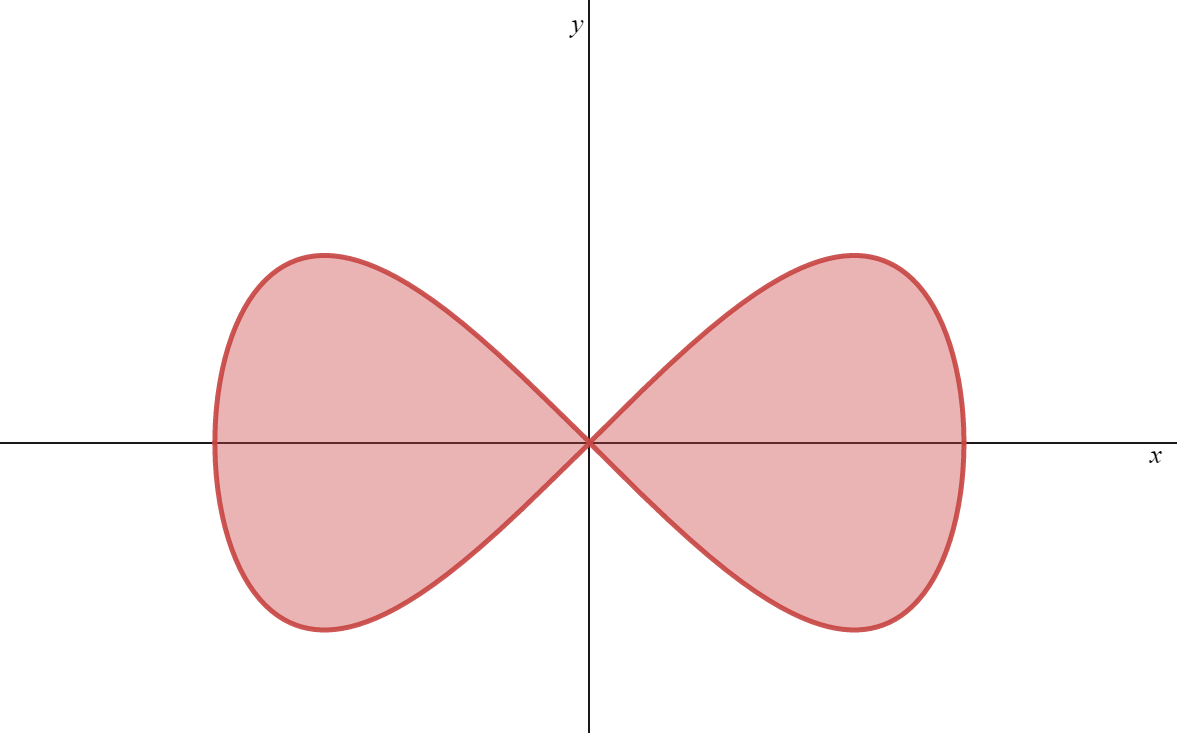
\includegraphics[width=0.6\textwidth]{Polar.png}
\end{figure}
\newblock\newline\textbf{(i)} Find the area of $R$.
\newline
\newline\textit{Solution:} The curve intersects the axes at $(-2,0), (0,0)$ and $(2,0)$. With simple algebraic manipulation, the top half of the curve can be represented by \[y=\sqrt{x^2-\frac{1}{4}x^4}.\] As such, due to symmetry, the area of $R$ is four times the integral over the top half of the curve from 0 to 2. That is, \begin{align*}
    \text{Area}&=4\int_{0}^{2}\sqrt{x^2-\frac{1}{4}x^4}\text{ }dx\\
    &=2\int_{0}^{2}\sqrt{4x^2-x^4}\text{ }dx\\
    &=2\int_{0}^{2}x\sqrt{4-x^2}\text{ }dx\\
    &=\frac{16}{3}\text{ units}^2
\end{align*}\qed
\newline\textbf{(ii)} Find the volume of the solid formed by rotating $R$ completely about the $x$-axis.
\newline
\newline\textit{Solution:} By the disk method, the volume is \begin{align*}
    \int_{-2}^{2}\pi y^2\text{ }dx&=\pi\int_{-2}^{2}x^2-\frac{1}{4}x^4\text{ }dx\\
&=\frac{32}{15}\pi\text{ units}^3    
\end{align*} \qed
\newline
\newline\textbf{(iii)} Find the volume of the solid formed by rotating $R$ completely about the $y$-axis.
\newline
\newline\textit{Solution:} By the shell method, the volume is \begin{align*}
    2\int_{0}^{2}2\pi xy\text{ }dx&=4\pi\int_{0}^{2}x\sqrt{x^2-\frac{1}{4}x^4}\text{ }dx\\
&=2\pi\int_{0}^{2}x^2\sqrt{4-x^2}\text{ }dx
\end{align*}
Using the substitution $x=2\operatorname{sin}\theta$, we have $dx=2\operatorname{cos}\theta\text{ }d\theta$, so the integral becomes \[2\pi\int_{0}^{\pi/2}4\operatorname{sin}^2\theta\cdot 2\operatorname{cos}\theta\cdot 2\operatorname{cos}\theta\text{ }d\theta=32\pi\int_{0}^{\pi/2}\operatorname{sin}^2\theta\operatorname{cos}^2\theta\text{ }d\theta=8\pi\int_{0}^{\pi/2}\operatorname{sin}^2 2\theta\text{ }d\theta.\] Using the identity $\operatorname{cos}4\theta=1-2\operatorname{sin}^2 2\theta$, it is easy to show that the volume is $2\pi^2$ units$^3$.\qed 
\newpage
\subsubsection*{Question 5}
A triangle is bounded by the tangent line to $y=e^x\text{ }(x<1)$ and the axes. Find the coordinates of the tangent point so that the triangle attains its largest area. Justify your answer.
\begin{figure}[h!]
\centering
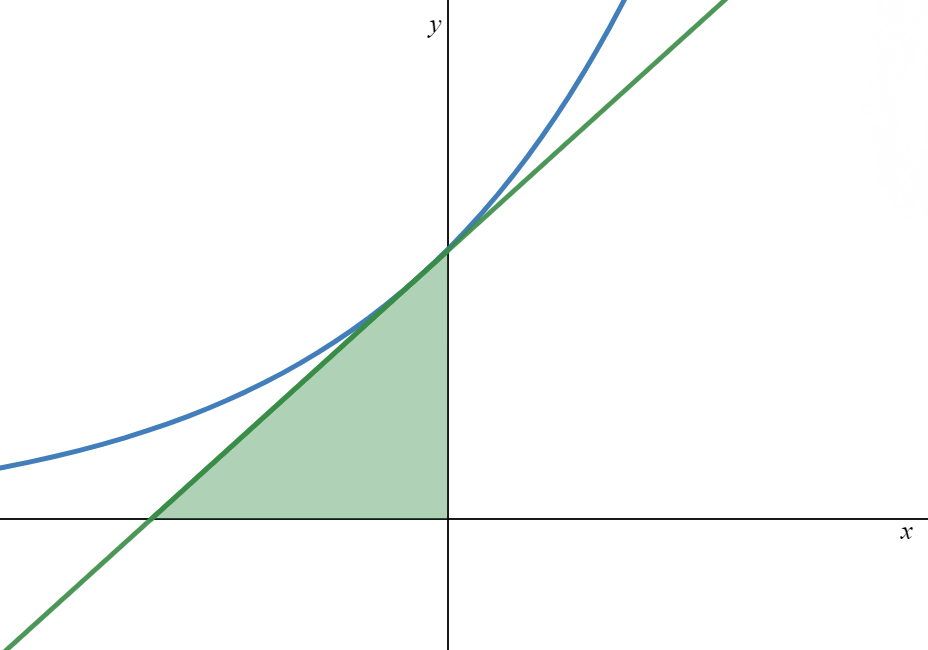
\includegraphics[width=0.6\textwidth]{ex.png}
\end{figure}
\newblock
\newline\textit{Solution:} Consider a point $P(a,e^a)$. The equation of the tangent to $P$ is \[y-e^a=e^a(x-a)\] so upon rearranging, \[y=e^ax-ae^a+e^a.\]
To find the $y$-intercept, set $x=0$, so $y=e^a(1-a)$. To find the $x$-intercept, set $y=0$, so $x=a-1$.
\newline\newline Thus, the tangent intersects the $y$-axis and $x$-axis at $(0,e^a(1-a))$ and $(a-1,0)$ respectively. The area of the triangle formed is \[\frac{1}{2}\cdot e^a(1-a) \cdot (1-a)=-\frac{e^a}{2}\cdot (1-a)^2\text{ as }a-1<0.\] Now, \[f'(a)=-\frac{e^a}{2}\cdot (a^2-1),\] so $f'(a)=0 \implies a=-1$ since $a<1$. One can use the first derivative test (the second derivative test fails here) to verify that at $P(-1,e^{-1})$, the area of the triangle formed is a maximum. \qed 
\newpage
\subsubsection*{Question 6}
\textbf{(i)} For $x \ge 1$, let $n=\lfloor{x}\rfloor$ and define \[f(x)=(n+1-x)\operatorname{ln}n+(x-n)\operatorname{ln}(n+1).\] Show that for all $x \ge 1$, $f(x) \le \operatorname{ln}x$ and that for all $n\in\mathbb{Z}^+$, \[\int_{1}^{n}f(x)\text{ }dx=\operatorname{ln}(n!)-\frac{1}{2}\operatorname{ln}n.\]
\textit{Solution:} Define $\left\{x\right\}$ to be the fractional part of the integer $x$. That is, $\left\{x\right\}=x-\lfloor{x}\rfloor$. So, 		\begin{align*}
   f\left( x \right)-\ln x&=(n+1-x)\ln n+(x-n)\ln (n+1)-\ln x \\ 
 & =\left( n-x \right)\left( \ln n-\ln \left( n+1 \right) \right)+\ln \left( \frac{n}{x} \right) \\ 
 & =\left( \left\lfloor x \right\rfloor -x \right)\left( \ln \left\lfloor x \right\rfloor -\ln \left( \left\lfloor x \right\rfloor +1 \right) \right)+\ln \left( \frac{\left\lfloor x \right\rfloor }{x} \right) \\ 
 & =\left( x-\left\lfloor x \right\rfloor  \right)\left( \ln \left( \left\lfloor x \right\rfloor +1 \right)-\ln \left\lfloor x \right\rfloor  \right)-\ln \left( \frac{x}{\left\lfloor x \right\rfloor } \right) \\ 
 & =\left\{ x \right\}\ln \left( 1+\frac{1}{\left\lfloor x \right\rfloor } \right)-\ln \left( \frac{\left\lfloor x \right\rfloor +\left\{ x \right\}}{\left\lfloor x \right\rfloor } \right) \\ 
 & =\left\{ x \right\}\ln \left( 1+\frac{1}{\left\lfloor x \right\rfloor } \right)-\ln \left( 1+\frac{\left\{ x \right\}}{\left\lfloor x \right\rfloor } \right)  
\end{align*}
If we can prove that \[\left\{ x \right\}\ln \left( 1+\frac{1}{\left\lfloor x \right\rfloor } \right)\le \ln \left( 1+\frac{\left\{ x \right\}}{\left\lfloor x \right\rfloor } \right),\] then we are done. This follows because \[{{\left( 1+\frac{1}{\left\lfloor x \right\rfloor } \right)}^{\left\{ x \right\}}}\le 1+\frac{\left\{ x \right\}}{\left\lfloor x \right\rfloor },\] which can be proven using Bernoulli's Inequality.
\begin{mybox}
    \textbf{Bernoulli's Inequality:} If $x\ge -1$ and $0\le r<1$, then $(1+x)^r\le 1+rx$.
\end{mybox}
As Bernoulli's Inequality states that $(1+x)^r \le 1+rx$, then replacing $x$ with $1/\left\lfloor x\right\rfloor$ and $r$ with $\left\{x\right\}$, the result follows. 
\newline
\newline The integral from $1$ to $n$ of $f(x)$ denotes the area under the curve from $x=1$ to $x=n$. From $x=1$ to $x=2$, the area under the curve is in the form of a triangle, whereas for all $x\in [a,a+1]$ where $a \ge 2$, the area under the curve in each interval takes the form of a trapezium.
\newline
\newline We try to find a pattern. The area under the curve from $x=1$ to $x=2$ is \[\frac{1}{2}\cdot 1 \cdot \operatorname{ln}2.\] The area under the curve from $x=2$ to $x=3$ is \[\frac{1}{2}\cdot 1 \cdot (\operatorname{ln}3+\operatorname{ln}2).\]
The area under the curve from $x=3$ to $x=4$ is \[\frac{1}{2}\cdot 1 \cdot (\operatorname{ln}4+\operatorname{ln}3).\] Hence, \begin{align*}
    \int_{1}^{n}f(x)\text{ }dx&=\frac{1}{2}\left( \ln 2+\ln 2+\ln 3+\ln 3+\ln 4+\ln 4+\ldots +\ln \left( n-1 \right)+\ln \left( n-1 \right)+\ln n \right)\\
    &=\frac{1}{2}\ln \left( n! \right)+\frac{1}{2}\ln \left( \left( n-1 \right)! \right)\\
    &=\ln \left( n! \right)-\frac{1}{2}\ln n
\end{align*} \qed
\newline
\newline\textbf{(ii)} For $x \ge 1$, let $n$ be the unique integer such that $n-1/2<x<n+1/2$ and define \[g(x)=\frac{x}{n}-1+\operatorname{ln}n.\]
Show that for all $x\ge 1$, $g(x)\ge \operatorname{ln}x$ and that for all $n \in \mathbb{Z}^+$, \[\int_{1}^{n}g(x)\text{ }dx=\int_{1}^{n}f(x)\text{ }dx+\frac{1}{8}\left(1-\frac{1}{n}\right).\]
\textit{Solution:} It suffices to show that $h(k)=k-1-\operatorname{ln}k\ge 0$ for $k \ge 0$. Note that $h(1)=0$ and $h'(k)=1-1/k$ so $h$ is an increasing function. The result follows.
\newline
\newline As for the integral, replace $n$ with $\lfloor{x}+1/2\rfloor$ so \[g(x)=\frac{x}{\lfloor{x+1/2}\rfloor}-1+\operatorname{ln}\left \lfloor {x+\frac{1}{2}} \right \rfloor.\] The area under $g$ from $x=1$ to $x=n$ comprises a triangle between $x=1$ and $x=1.5$ and a trapezium between $x=3/2$ and $x=5/2$, as well as between $x=5/2$ and $x=7/2$, and so on.
\newline
\newline The area of the triangle is \[\frac{1}{2}\cdot \frac{1}{2} \cdot \frac{1}{2} =\frac{1}{8}.\]
The area of the trapezium bounded between $y=g(x)$ and the ordinates $x=3/2$ and $x=5/2$ is 
\[\frac{1}{2}\cdot 1 \cdot \left(\frac{3}{4}-1+\ln\left(2\right)+\frac{1}{4}+\ln2 \right )=\operatorname{ln}2.\]
As such, it is easy to see that the area of the trapezium bounded between $y=g(x)$ and the ordinates $x=5/2$ and $x=7/2$ is $\operatorname{ln}3$.
\newline
\newline However,  the upper bound of the integral of $g$ is $n$, which is an integer. Based on the pattern established earlier, \[\int_{n-1/2}^{n+1/2}g(x)\text{ }dx=\operatorname{ln}n,\] but the integral from $n$ to $n+1/2$ should be omitted. This is the area of another trapezium, which is \begin{align*}
  & \frac{1}{2}\underbrace{\left( n+\frac{1}{2}-n \right)}_{\text{width}}\underbrace{\left[ g\left( n \right)+g\left( n+\frac{1}{2} \right) \right]}_{\text{sum of parallel sides}}=\frac{1}{4}\left[ g\left( n \right)+g\left( n+\frac{1}{2} \right) \right] \\ 
 & =\frac{1}{4}\left( \frac{n}{n}-1+\ln n+\frac{n+1/2}{n}-1+\ln n \right) \\ 
 & =\frac{1}{4}\left( 2\ln n+\frac{1}{2n} \right)  
\end{align*}
In a similar fashion as compared to \textbf{(i)}, \begin{align*}
    \int_{1}^{n}g(x)\text{ }dx&=\frac{1}{8}+\operatorname{ln}2+\operatorname{ln}3+\hdots+\operatorname{ln}n-\frac{1}{4}\left(2\operatorname{ln}n+ \frac{1}{2n}\right)\\
    &=\frac{1}{8}+\operatorname{ln}1+\operatorname{ln}2+\operatorname{ln}3+\hdots+\operatorname{ln}n-\frac{1}{4}\left(2\operatorname{ln}n+ \frac{1}{2n}\right)\\
    &=\frac{1}{8}+\operatorname{ln}(n!)-\frac{1}{2}\operatorname{ln}n-\frac{1}{8n}\\
    &=\operatorname{ln}(n!)-\frac{1}{2}\operatorname{ln}n+\frac{1}{8}\left(1-\frac{1}{n}\right)
\end{align*}\qed
\newline
\newline
\textbf{(iii)} Use the results in \textbf{(i)} and \textbf{(ii)} to conclude that for all $n\in\mathbb{Z}^+$, \[\frac{7}{8}\le \operatorname{ln}(n!) -\left(n+\frac{1}{2}\right)\operatorname{ln}n+n\le 1.\]
\textit{Solution:} First, set \[q=\operatorname{ln}(n!) -\left(n+\frac{1}{2}\right)\operatorname{ln}n+n.\]
Note that \[q=\ln (n!)-\frac{1}{2}\ln n+n\left( 1-\ln n \right)=\int_{1}^{n}{f\left( x \right)\text{ }dx}+n\left( 1-\ln n \right).\] Since $f(x) \le \operatorname{ln}x$ from \textbf{(i)}, then \[\int_{1}^{n}f(x)\text{ }dx \le \int_{1}^{n}\operatorname{ln}x\text{ }dx=n\operatorname{ln}n-n+1.\] It is thus clear that an upper bound for $q$ is obtained, and that is 1.
\newline
\newline Using \textbf{(ii)}, since $g(x)\ge \operatorname{ln}x$, then \[\int_{1}^{n}g(x)\text{ }dx\ge \int_{1}^{n}\operatorname{ln}x\text{ }dx=n\operatorname{ln}n-n+1.\]
From \textbf{(ii)}, we showed that \[\int_{1}^{n}g(x)\text{ }dx=\int_{1}^{n}f(x)\text{ }dx+\frac{1}{8}\left(1-\frac{1}{n}\right).\]
Thus, \[\int_{1}^{n}f(x)\text{ }dx \ge \frac{1}{8}\left(\frac{1}{n}-1\right)+n\operatorname{ln}n-n+1.\] Hence, \[q \ge n-n\operatorname{ln}n+\frac{1}{8n}-\frac{1}{8}+n\operatorname{ln}n-n+1=\frac{7}{8}+\frac{1}{8n}\ge \frac{7}{8},\] so a lower bound for $q$ is obtained, which is $7/8$. \qed 
\newline
\newline
\textbf{(iv)} Use the results in \textbf{(iii)} to conclude that \[e^{7/8} \le \frac{n!}{(n/e)^n\sqrt{n}}\le e.\]
\textit{Solution:} \begin{align*}
   q&=\ln (n!)-\left( n+\frac{1}{2} \right)\ln n+n \\ 
 & =\ln (n!)-\ln \left( {{n}^{\left( 2n+1 \right)/2}} \right)+\ln \left( {{e}^{n}} \right) \\ 
 & =\ln \left( \frac{{{e}^{n}}n!}{{{n}^{\left( 2n+1 \right)/2}}} \right)  
\end{align*}
Since $q$ is bounded between $7/8$ and 1, we have \[e^{7/8} \le \frac{{{e}^{n}}n!}{{{n}^{\left( 2n+1 \right)/2}}} \le e.\]
The term that is sandwiched here is indeed the one given at the start of the question, so we are done. \qed 
\newline
\newline \textbf{\textcolor{purple}{REMARK:}} The interested can search up Stirling's Approximation for a related beautiful result.
\newpage
\subsubsection*{Question 7}
\textbf{(a)} Consider the following initial value problem: \[\frac{dy}{dx}=2e^{-x}y^2+2y-3e^x,\text{ where }y=0\text{ at }x=0.\]
\textbf{(i)} Use the substitution $y=e^x+1/z$ to convert the differential equation of the given initial value problem into a first order linear equation in $x$ and $z$.
\newline
\newline\textit{Solution:} The substitution yields \[\frac{dy}{dx}={{e}^{x}}-{{z}^{-2}}\frac{dz}{dx}\] so the differential equation becomes \begin{align*}
   2{{e}^{-x}}{{\left( {{e}^{x}}+\frac{1}{z} \right)}^{2}}+2\left( {{e}^{x}}+\frac{1}{z} \right)-3{{e}^{x}}&={{e}^{x}}-{{z}^{-2}}\frac{dz}{dx} \\ 
  2{{e}^{-x}}\left( {{e}^{2x}}+\frac{2{{e}^{x}}}{z}+{{z}^{-2}} \right)+2{{e}^{x}}+2{{z}^{-1}}&=4{{e}^{x}}-{{z}^{-2}}\frac{dz}{dx} \\ 
  \frac{dz}{dx}+6z&=-2{{e}^{-x}}  
\end{align*}\qed 
\newline
\newline
\textbf{(ii)} Solve the differential equation obtained in \textbf{(i)}. Hence, solve the initial value problem. Express
the answer as $y=f(x)$.
\newline
\newline  The integrating factor is \[e^{\int 6\text{ }dx}=e^{6x},\] hence multiplying both sides by the integrating factor, we have \[\frac{d}{dx}\left(ze^{6x}\right)=-2e^{5x}.\] Thus, \[ze^{6x}=-\frac{2}{5}e^{5x}+c.\] When $x=y=0$, then $z=-1$, so $c=3/5$. Hence, \[y=-\frac{3e^x(e^{5x}-1)}{2e^{5x}+3}.\] \qed 
\newline
\newline \textbf{(b)} Let $f$ be a function that is non-negative, increasing and continuous on $[0,2]$, and differentiable on $(0,2)$. A surface $S$ is formed by rotating the curve $y=f(x)$ completely about the $x$-axis.
Suppose that the area of the portion of $S$ on any interval $[a,b] \subseteq [0,2]$ is always $10\pi(b-a)$. If
$f(0) = 3$, find the expression for $f(x)$.
\newline
\newline\textit{Solution:} Using the formula for the surface area of revolution, \[\int_{0}^{x}{2\pi f\left( t \right)\sqrt{1+{{\left( f'\left( t \right) \right)}^{2}}}\text{ }dt}=10\pi x,\] where $a=0$ and $b=x$ and $[a,b]\subseteq [0,2]$. By the First Fundamental Theorem of Calculus, differentiating both sides, \[2\pi f(x)\sqrt{1+(f'(x))^2}=10\pi.\] The differential equation becomes \begin{align*}
  f(x)\sqrt{1+{{({f}'(x))}^{2}}}&=5 \\ 
  {{\left( f(x) \right)}^{2}}+{{\left( f(x){f}'(x) \right)}^{2}}&=25  
\end{align*} Using the substitution $u(x)=(f(x))^2$, we have $u'(x)=2f(x)f'(x)$, so the differential equation becomes \[u(x)+\frac{1}{4}(u'(x))^2=25.\] Differentiating both sides, \[u'(x)\left(1+\frac{1}{2}u''(x)\right)=0.\] Either $u'(x)=0$ or $u''(x)=-2$. The former yields $u(x)=c_1$, so $f(x)=\pm\sqrt{c_1}$. Since $f(0)=3$, this solution yields $f(x)=3$ for all $0 \le x \le 2$. However, substituting this into the surface area of revolution formula, for $a \le x \le b$, \[\int_{a}^{b} 2\pi \cdot 3\text{ }dx =6\pi (b-a) \ne 10\pi (b-a).\] As such, we consider the latter of the two solutions, for which it yields $u(x)=-x^2+c_2x+c_3$, so $f(x)=\pm\sqrt{-x^2+c_2x+c_3}$, but since $f$ is non-negative, then $f(x)=\sqrt{-x^2+c_2x+c_3}$. Substituting $f(0)=3$ gives $c_3=9$. Substituting $f(x)=\sqrt{-x^2+c_2x+9}$ into the surface area of revolution formula, for $a \le x \le b$, \[\int_{a}^{b} 2\pi \sqrt{-x^2+c_2x+9}\cdot \sqrt{1+\left(\dfrac{c_2-2x}{2\sqrt{-x^2+c_2x+9}} \right )^2}=10\pi(b-a).\] Thus, \begin{align*}
    \int_{a}^{b}\sqrt{-4x^2+4c_2x+36+c_2^2+4x^2-4c_2x}\text{ }dx&=10(b-a)\\
    \int_{a}^{b}\sqrt{36+c_2^2}\text{ }dx&=10(b-a)
\end{align*}
so $c_2=8$. We reject $c_2=-8$ because if $f(x)=\sqrt{-x^2-8x+9}$, then the domain of $f$ in this case does not include values of $x$ for $x>1$. Hence, we conclude that $f(x)=\sqrt{-x^2+8x+9}$. \qed
\newline
\newline \textbf{\textcolor{purple}{REMARK:}} There is some semblance to solving this differential equation as compared to Clairaut's Equation, for which the latter is given by \[y(x)=x\frac{dy}{dx}+f\left(\frac{dy}{dx}\right).\]
\newpage
\subsubsection*{Question 8}
Let $f$ be an increasing continuous function on $\mathbb{R}$ such that \[\lim_{x\rightarrow\infty}\frac{1}{x}\int_{0}^{x}f(t)\text{ }dt=1.\] Prove that $\lim_{x\rightarrow\infty}f(x)$ exists and equals 1.
\newline\newline\textit{Solution:} We are given an increasing, continuous real-valued function $f$ such that:\[\lim_{x\to\infty}\frac1x\int^x_0f(t)\text{ }dt=1.\]
Suppose the limit of $f(x)$ when $x$ tends to infinity does not exist. Since $f$ is increasing, this means that as $x$ increases, $f$ will always increase and never level off from some value of $x$ onwards. In other words, $\displaystyle \lim_{x\to\infty} = +\infty.$ Then, $\displaystyle\int^x_0f(t)\text{ }dt=+\infty $. However, this means that
\begin{align*}
    \lim_{x\to\infty}\frac{1}{x}\int_{0}^{x}f(t)\text{ }dt&=\lim_{x\to\infty}f(x) \ \ \ \text{by L'Hôpital's Rule}\\ &= +\infty
\end{align*}
which is a contradiction. Thus, the limit $\displaystyle\lim_{x\to\infty}f(x)$ exists.
\newline
\newline
Suppose $\displaystyle\lim_{x\to\infty}f(x)<1$. This means that for all real values of $x$, $f(x)<1$. However, this means that
\begin{align*}
   \lim_{x\rightarrow\infty}\frac{1}{x}\int_{0}^{x}f(t)\text{ }dt&<\lim_{x\to\infty}\frac{1}{x}\int_{0}^{x}dt\\
    &=\lim_{x\to\infty}\frac{x}{x}\\&=1
\end{align*}
which is a contradiction.
\newline
\newline Suppose $\displaystyle\lim_{x\to\infty}f(x)>1$. Then, there exists $M\ge 0$ such such that for all $x>M$, $f(x)>1$ since $f$ is increasing and continuous. Then, denote a constant \[K = \int^M_0f(t)\text{ }dt.\]
Thus, 
\begin{align*}
\lim_{x\to\infty}\int^x_0f(t)\text{ }dt =  \lim_{x\to\infty}\left(K+\int^x_M f(t) \text{ }dt \right)= +\infty
\end{align*}
because for $x>M$,
\begin{align*}
    \int^x_M f(t)\text{ } dt &>\int^x_M dt = x-M \\
    \lim_{x\to\infty}\int^x_M f(t) \text{ }dt &= \lim_{x\to\infty}(x-M) = +\infty
\end{align*}
so by L'Hôpital's Rule,
\begin{align*}
    \lim_{x\to\infty}\frac{1}{x}\int_0^xf(t)\text{ }dt&= \lim_{x\to\infty}f(x) \\ &>1
\end{align*}
which is a contradiction.
\newline
\newline Thus, we conclude that the limit exists, and must be equal to 1. \qed 
\end{document}
